\chapter{[Kapitel]}
Formatvorlage für den Fließtext. Formatvorlage für den Fließtext. Formatvorlage für den Fließtext. Formatvorlage für den Fließtext. Formatvorlage für den Fließtext. Formatvorlage für den Fließtext. Formatvorlage für den Fließtext. Formatvorlage für den Fließtext. Formatvorlage für den Fließtext. Formatvorlage für den Fließtext. Formatvorlage für den Fließtext.
\begin{quote}
  Formatvorlage für ein längeres direktes Zitat. Formatvorlage für ein längeres direktes Zitat. Formatvorlage für ein längeres direktes Zitat. Formatvorlage für ein längeres direktes Zitat. Formatvorlage für ein längeres direktes Zitat. Formatvorlage für ein längeres direktes Zitat….
\end{quote}

Formatvorlage für den Fließtext.
Hier eine Liste.
\begin{enumerate}
 \item Verstehen
 \item Üben
 \item Können
\end{enumerate}


\section{[Unterkapitel zweite Ebene]}
Formatvorlage für den Fließtext. Die Abbildung~\ref{fig:ex} auf Seite~\pageref{fig:ex} zeigt drei Entladungskurven eines biphasischen Defibrillators.
\begin{figure}[htb]
  \centering
  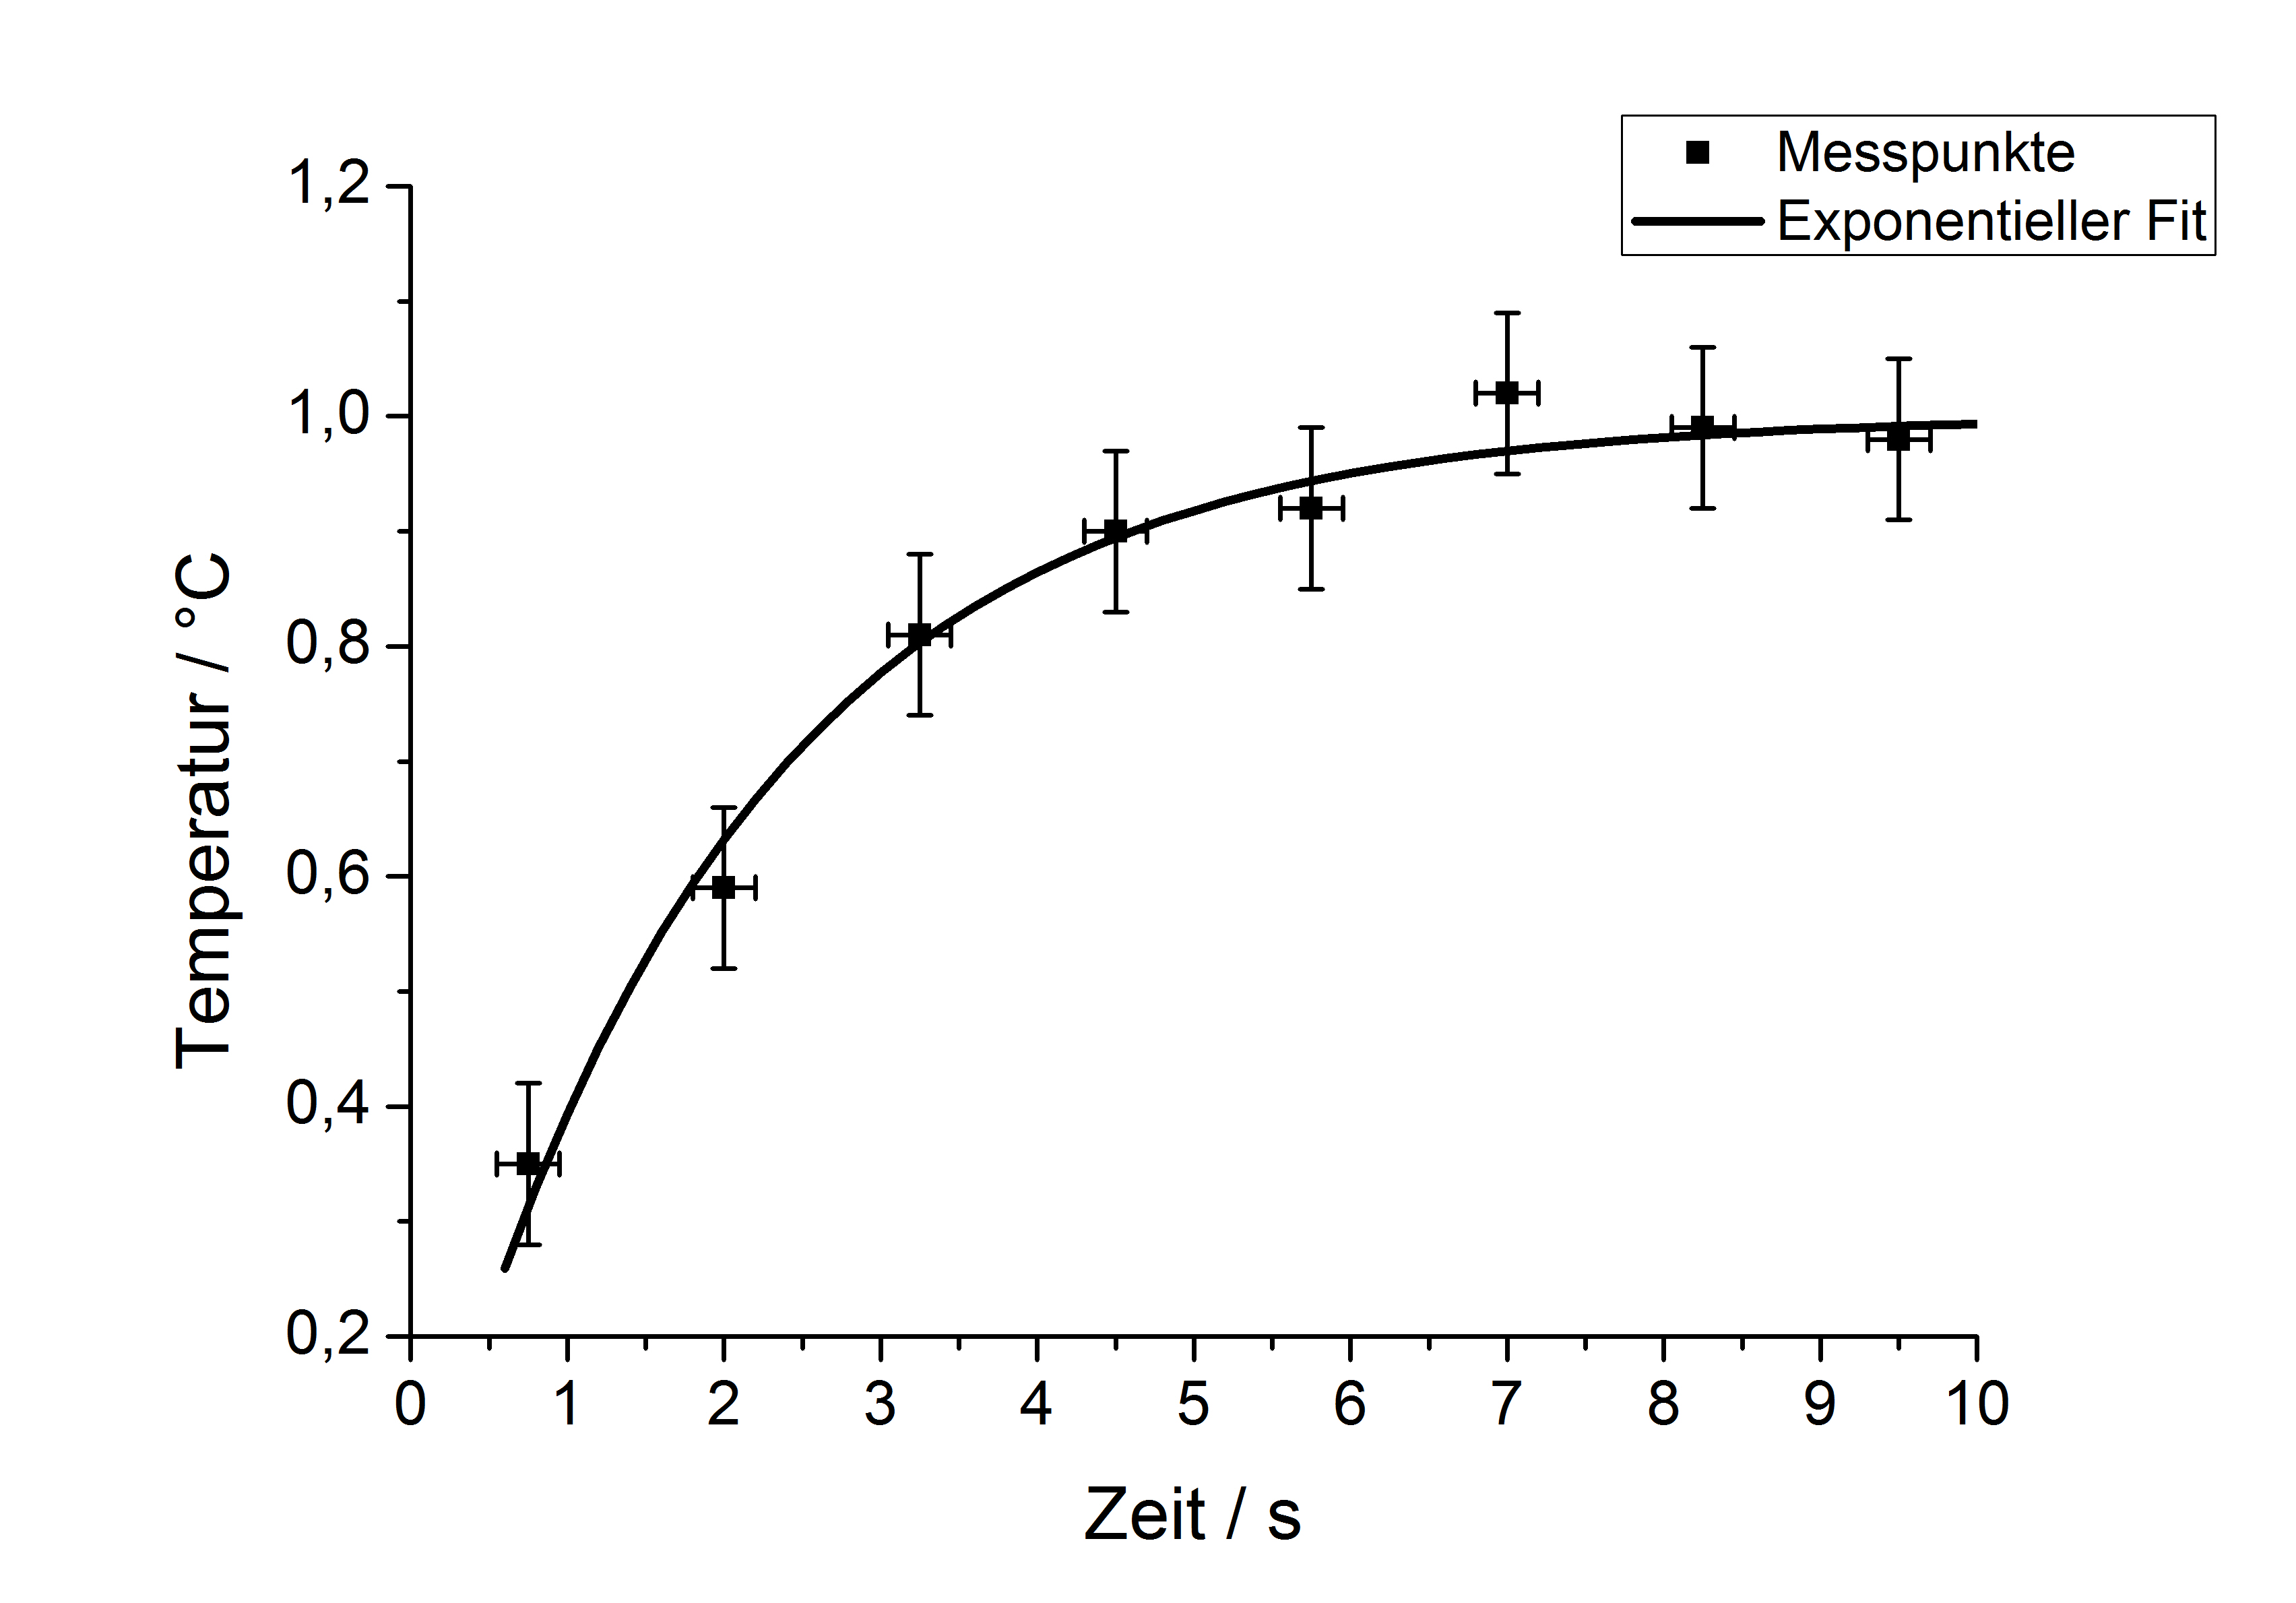
\includegraphics[width=10cm]{Amann_TechnAbb}
  \caption[Aufheizverhalten von PTFE]{Das Bild zeigt das Aufheizverhalten von PTFE\@. \\Quelle: eigene Ausarbeitung}
\label{fig:ex}
\end{figure}


\section{[Unterkapitel zweite Ebene]}
Formatvorlage für den Fließtext.
Jetzt eine Fußnote\footnote{Dies ist eine Fußnote.}
Die quadratischen Gleichung (\ref{equ:foo}) hat wieviele Nullstellen?
\begin{equation}
 \label{equ:foo}
 x^2-2x+5=0.
\end{equation}
Zwei von Einsteins berühmtesten Formeln lauten:
\begin{eqnarray*}
  E &= mc^2                                  \\
  m &= \frac{m_0}{\sqrt{1-\frac{v^2}{c^2}}}
\end{eqnarray*}


\subsection{[Unterkapitel dritte Ebene]}
Formatvorlage für den Fließtext. Hier die einfache Tabelle~\ref{tab:sp}

\begin{table}[htb]
  \centering
  \begin{tabular}{ | l | l |c|}
    \hline
    Datum      & Thema           & Raum \\
    \hline\hline
    Montag     & Graphentheorie  & U1   \\
    \hline
    Donnerstag & Algebra         & MZB23\\
    \hline
  \end{tabular}
  \caption[Stundenplan]{Stundenplan des Jahres 2030.\\Quelle: eigene Ausarbeitung}
\label{tab:sp}
\end{table}

\subsubsection{[Unterkapitel vierte Ebene]}
Formatvorlage für den Fließtext.



\section{[Unterkapitel zweite Ebene]}

Verweise: zu einem Buch mit Details~\cite[vgl.][Kapitel 2]{bathe_finite-elemente-methoden_1990} oder ohne Details~\cite{bathe_finite-elemente-methoden_1990}, ein Buchteil~\cite{areger_problem-based_2007}, eine Dissertation~\cite{sporn_interaktives_2000}, ein Dokument~\cite{industriellenvereinigung_beste_2014}, ein Enzyklopädieartikel~\cite{brockhaus_kreativitat_1872}, ein Film~\cite{de_wilde_through_2008}, ein Konferenz-Paper~\cite{weber_podcasts._2006}, ein Magazin-Artikel~\cite{autornachname1_magazinartikeltitel_1995}, ein Pordcast~\cite{paulus_horen_????}, eine Tonaufnahme~\cite{horowitz_horowitz_2003}, eine Videoaufnahme~\cite{fhvlearningsupport_was_2008}, ein Vortrag~\cite{kohls_literaturverwaltung_2008}, eine Website~\cite{wedekind_von_2008}, ein Zeitschriftenartikel~\cite{hofer_wir_2008} und ein Zeitungsartikel~\cite{schenkel_tsunami_2012}.


\chapter{[Kapitel]}

\section{[Unterkapitel zweite Ebene]}
Formatvorlage für den Fließtext.

\subsection{[Unterkapitel dritte Ebene]}
Formatvorlage für den Fließtext.

\subsubsection{[Unterkapitel vierte Ebene]}
Formatvorlage für den Fließtext.
